\documentclass[journal]{IEEEtran} % use the `journal` option for ITherm conference style
\IEEEoverridecommandlockouts
% The preceding line is only needed to identify funding in the first footnote. If that is unneeded, please comment it out.
\usepackage{cite}
\usepackage{amsmath,amssymb,amsfonts}
\usepackage{graphicx}
\usepackage{textcomp}
\usepackage{xcolor}
\usepackage{svg}

\usepackage{hyperref}
\usepackage{float}
\usepackage{tikz}
\usepackage{circuitikz}
\usepackage[sort&compress,numbers]{natbib}
%\bibliographystyle{dinat}
%\bibliographystyle{IEEEtranN}
\bibliographystyle{myIEEEtran}
\usepackage{amsmath}
\usepackage{fontawesome5}
\usepackage{rotating}
\usepackage{pifont}


\usepackage{algorithm}
\usepackage[noend]{algpseudocode}
\usepackage{tabularx}
\usepackage{xltabular}
\usepackage{longtable}
\usepackage{makecell}

\usepackage{lineno}
\usepackage{todonotes}

\makeatletter
\def\BState{\State\hskip-\ALG@thistlm}
\makeatother

\makeatletter
\def\BState{\State\hskip-\ALG@thistlm}
\makeatother

\usepackage{helvet}
\usepackage{tabularray}

\usetikzlibrary{shapes}
\usetikzlibrary{arrows}

\tikzstyle{every task} = []
\tikzstyle{every gateway} = []
\tikzstyle{every sequence} = []
\tikzstyle{every message} = []
\tikzstyle{every association} = []
\tikzstyle{every event} = []

\tikzstyle{task} = [rectangle, draw, black,
minimum width=4em, minimum height=2em,rounded corners,align=center,every task]

\tikzstyle{gateway} = [diamond, draw, black,inner sep=0pt,minimum width=2.5em, minimum height=2.5em,every gateway]
\tikzstyle{sequence} = [->,>=triangle 45,every sequence]
\tikzstyle{message} = [o->,dashed,>=open triangle 45,every sequence]
\tikzstyle{association} = [->,densely dotted,>=angle 45,every association]
\tikzstyle{event} = [circle,minimum width=1.5em, minimum height=1.5em,draw,every event]
\tikzstyle{end event} = [event,ultra thick,every event]
\tikzstyle{intermediate event} = [event,double,every event]

%Center in tables
\newcommand\addvmargin[1]{
  \node[fit=(current bounding box),inner ysep=#1,inner xsep=0]{};
}

\newcommand\centerTable[1]{
    \begin{tikzpicture}[baseline=0]
             \node[](a){};
            \node[above=0.1cm of a](e){#1};
            \node[above=0.1cm of e](b){};
        \end{tikzpicture}
}

% Keywords command
\providecommand{\keywords}[1]
{
	\begin{center}
		\small	
		\textbf{Keywords} 
	\end{center}
	\begin{center}
		#1
	\end{center}
}
\usetikzlibrary{arrows.meta, automata,
	calc,
	positioning,
	quotes,
	fit}

\tikzstyle{mybox} = [draw,rectangle, minimum height=0.75cm,minimum width=4cm]

\newcommand{\vertices}{V}
\newcommand{\edges}{E}
\newcommand{\executables}{T}
\newcommand{\model}{M}
\newcommand{\vect}{v}

\newcommand{\hcurr}{h_{current}}
\newcommand{\hnew}{h_{new}}
\newcommand{\hnext}{h_{next}}

\newcommand{\scurr}{s_{current}}
\newcommand{\snew}{s_{new}}
\newcommand{\snext}{s_{next}}

\newcommand{\Scurr}{S_{current}}
\newcommand{\Snew}{S_{new}}
\newcommand{\Snext}{S_{next}}

\newcommand{\rcurr}{r_{current}}
\newcommand{\rnew}{r_{new}}
\newcommand{\rnext}{r_{next}}



\newcommand{\Ccurr}{C^{enc}_{curr}}
\newcommand{\Cnew}{C^{enc}_{new}}
\newcommand{\Cnext}{C^{enc}_{next}}

\newcommand{\sk}{sk}
\newcommand{\pk}{pk}
\newcommand{\proof}{proof}

\def\BibTeX{{\rm B\kern-.05em{\sc i\kern-.025em b}\kern-.08em
    T\kern-.1667em\lower.7ex\hbox{E}\kern-.125emX}}
\begin{document}

\title{Blockchain-Based, Confidentiality-Preserving Orchestration of Collaborative Workflows}
% delete or comment-out the following line before submission
%{\footnotesize \textsuperscript{*}Note: Sub-titles are not captured in Xplore and should not be used}
%\thanks{Identify applicable funding agency here. If none, delete this.}
%}

\author{%%%% author names
    \IEEEauthorblockN{Bal\'{a}zs \'{A}d\'{a}m Toldi}% first author
    , \IEEEauthorblockN{Imre Kocsis}% delete this line if not needed
    %, \IEEEauthorblockN{3\textsuperscript{rd} Given Name Surname}% delete this line if not needed
    % duplicate the line above as many times as needed to list all authors
    \\%%%% author affiliations
    \IEEEauthorblockA{\textit{Dept. of Measurement and Information Systems\\ Budapest University of Technology and Economics\\Budapest, Hungary}}\\% first affiliation
    %\IEEEauthorblockA{\textit{Department of Measurement and Information Systems --- Budapest University of Technology and Economics}}\\% delete this line if not needed
    % duplicate the line above as many times as needed to list all affiliations
    %%%% corresponding author contact details
    \IEEEauthorblockA{balazs.toldi@edu.bme.hu, kocsis.imre@vik.bme.hu}
}

\maketitle



Over the past few years, there has been a significant amount of research focused on studying the ReLU activation function, with the aim of achieving neural network convergence through over-parametrization. However, recent developments in the field of Large Language Models (LLMs) have sparked interest in the use of exponential activation functions, specifically in the attention mechanism.

Mathematically, we define the neural function $F: \R^{d \times m} \times  \mathbb{R}^d \rightarrow \mathbb{R}$ using an exponential activation function. Given a set of data points with labels $\{(x_1, y_1), (x_2, y_2), \dots, (x_n, y_n)\} \subset \mathbb{R}^d \times \mathbb{R}$ where $n$ denotes the number of the data. Here $F(W(t),x)$ can be expressed as $F(W(t),x) := \sum_{r=1}^m a_r \exp(\langle w_r, x \rangle)$, where $m$ represents the number of neurons, and $w_r(t)$ are weights at time $t$. It's standard in literature that $a_r$ are the fixed weights and it's never changed during the training. We initialize the weights $W(0) \in \mathbb{R}^{d \times m}$ with random Gaussian distributions, such that $w_r(0) \sim \mathcal{N}(0, I_d)$ and initialize $a_r$ from random sign distribution for each $r \in [m]$.

Using the gradient descent algorithm, we can find a weight $W(T)$ such that $\| F(W(T), X) - y \|_2 \leq \epsilon$ holds with probability $1-\delta$, where $\epsilon \in (0,0.1)$ and $m = \Omega(n^{2+o(1)}\log(n/\delta))$. To optimize the over-parametrization bound $m$, we employ several tight analysis techniques from previous studies [Song and Yang arXiv 2019, Munteanu, Omlor, Song and Woodruff ICML 2022]. 

 


\section{Introduction}
\label{sec:introduction}
% \begin{itemize}
%     % Diffusion of FL
%     \item {\st{Diffusion of FL}}
%     % Security threats to FL
%     \item {\st{Security threats to FL with particular focus on model poisoning}}
%     % Limitations of existing countermeasures
%     \item {\st{Current countermeasures (e.g., KRUM) and their limitations}}
%     % Proposed method and its advantages
%     \item {\st{Intuitive description of the proposed method and its difference (i.e., advantages) w.r.t. state of the art}}
%     % Main contributions
%     \item {\st{Summary of the main contributions of this work}}
%     % Paper's structure and organization
%     \item {\st{Paper's structure and organization}}
% \end{itemize}

% Diffusion of FL
Recently, {\em federated learning} (FL) has emerged as the leading paradigm for training distributed, large-scale, and privacy-preserving machine learning (ML) systems~\cite{mcmahan2017googleai,mcmahan2017aistats}. 
The core idea of FL is to allow multiple edge clients to collaboratively train a shared, global model without disclosing their local private training data.
%Specifically, an FL system consists of a central server and many edge clients; 
A typical FL round involves the following steps: {\em(i)} the server randomly picks some clients and sends them the current, global model; {\em(ii)} each selected client locally trains its model with its own private data; then, it sends the resulting local model to the server;\footnote{Whenever we refer to global/local model, we mean global/local model {\em parameters}.} {\em(iii)} the server updates the global model by computing an \emph{aggregation function}, usually the average (FedAvg), on the local models received from clients.
% \begin{enumerate}
%     \item[{\em(i)}] the server sends the current, global model to the clients and appoints some of them for training;
%     \item[{\em(ii)}] each selected client locally trains its copy of the global model with its own private data; then, it sends the resulting local model back to the server;\footnote{Whenever we refer to global/local model, we mean global/local model {\em parameters}.}
%     \item[{\em(iii)}] the server updates the global model by computing an \emph{aggregation function} on the local models received from clients (by default, the average, also referred to as FedAvg~\cite{mcmahan2017aistats}).
% \end{enumerate}
This process goes on until the global model converges. %(e.g., after a certain number of rounds or other similar stopping criteria).
%\\
% The advantages of FL over the traditional, centralized learning paradigm are undoubtedly clear in terms of flexibility/scalability (clients can join/disconnect from the FL network dynamically), network communications (only model weights\footnote{We will use \textit{parameters} and \textit{weights} interchangeably.} are exchanged between clients and server), and privacy (each client's private training data is kept local at the client's end and not uploaded to the server).
\\
% Security threats to FL
%However, the growing adoption of FL also raises security concerns~\cite{costa2022covert}, particularly about its confidentiality, integrity, and availability.
Although its advantages over standard ML, FL also raises security concerns~\cite{costa2022covert}. %, particularly about its confidentiality, integrity, and availability~\cite{costa2022covert}.
% OLD, LONG VERSION
% Indeed, some work deals with privacy leakage that may expose the local data of some clients~\cite{melis2019sp}. 
% A large body of work, instead, investigates attacks that usually aim to detriment the predictive accuracy of the learned global model. For instance, \emph{data poisoning} attacks achieve this goal by letting an adversary pollute the training set of some corrupt FL clients with maliciously crafted examples~\cite{jagielski2018sp}.
% Similarly, in \emph{model poisoning} the attacker attempts to tweak the global model weights~\cite{bhagoji2019pmlr} by directly perturbing the local model's weights of some infected FL clients before these are sent to the central server for aggregation, usually via so-called Byzantine attacks. 
% It turns out that Byzantine model poisoning attacks severely impact standard FedAvg; therefore, more robust aggregation functions must be designed to make FL systems secure.
Here, we focus on \emph{untargeted model poisoning} attacks~\cite{bhagoji2019pmlr}, where an adversary attempts to tweak the global model weights %\footnote{We will use the terms \textit{parameters} and \textit{weights} interchangeably.} 
by directly perturbing the local model's parameters of some infected clients before these are sent to the central server for aggregation.
In doing so, the adversary aims to jeopardize the global model \textit{indiscriminately} at inference time.
Such model poisoning attacks severely impact standard FedAvg; therefore, more robust aggregation functions must be designed to secure FL systems.
\\
% In this paper, we focus on designing a novel robust aggregation scheme at the server's end to contrast the effect of Byzantine model poisoning attacks.
%
% Current countermeasures and their limitations
%Several countermeasures have been proposed in the literature to combat model poisoning attacks on FL systems.
% Some methods use simple statistics more robust than plain average to smooth the impact of malicious updates (e.g., Trimmed Mean and FedMedian~\cite{yin2018icml}). 
% Other defenses implement outlier detection techniques to discard malicious updates from the aggregation performed at the server's end. Those are either based on heuristics (e.g., Krum/Multi-Krum~\cite{blanchard2017nips} and Bulyan~\cite{mhamdi2018pmlr}) or data-driven approaches (e.g., K-means clustering~\cite{shen2016acm} or DnC via spectral analysis~\cite{shejwalkar2021ndss}). 
% Finally, some strategies rely on a centralized ``source of trust'' to spot potential malicious updates (e.g., FLTrust~\cite{cao2020fltrust}).
% Several countermeasures have been proposed in the literature to combat model poisoning attacks on FL systems, i.e., to discard possible malicious local updates from the aggregation performed at the server's end. 
% These techniques range from simple statistics more robust than plain average (e.g., Trimmed Mean and FedMedian~\cite{yin2018icml}) to outlier detection heuristics (e.g., Krum/Multi-Krum~\cite{blanchard2017nips} and Bulyan~\cite{mhamdi2018pmlr}) or data-driven approaches (e.g., spectral analysis via K-means clustering~\cite{shen2016acm} or spectral analysis), or methods based on ``source of trust'' (e.g., FLTrust~\cite{cao2020fltrust}).
% OLD, LONG VERSION
%Several countermeasures have been proposed in the literature to combat Byzantine model poisoning attacks on FL systems.
% Descriptive statistics
% For example, Trimmed Mean and FedMedian aggregate local model updates using more robust statistics than standard average~\cite{yin2018icml}.
%
% % Heuristics for outlier detection
% Many existing Byzantine-resilient strategies implement some outlier detection heuristics to discard the model updates sent by potentially malicious clients from the input of the aggregation function.
% One of the most popular heuristics is Krum~\cite{blanchard2017nips}.
% This strategy tries to mitigate the impact of Byzantine attacks by selecting as a global model the local model with the smallest sum of Euclidean distances to {\em all} the other local models.
% Although powerful, Krum requires the server to know (or, at least, estimate) the number of malicious FL clients upfront, which is generally impossible in a realistic attack scenario. %
% Moreover, Krum may become ineffective for complex, high-dimensional model parameter spaces due to the curse of dimensionality.
% Bulyan~\cite{mhamdi2018pmlr} tries to overcome this issue by combining Krum with a variant of Trimmed Mean.
% % Data-driven outlier detection
% Other strategies use data-driven outlier detection techniques -- e.g., via K-means clustering~\cite{shen2016acm} -- to spot potential malicious local model updates. 
% %For instance, Shen et al. propose to cluster local model updates with K-means and thus identify outliers.
%
% % Other techniques
% As far as the server is concerned, any local model received can be from a potential malicious client. 
% FLTrust~\cite{cao2020fltrust} assumes the server acts as a client, i.e., trains a local model on an additional {\em trustworthy} dataset at the server's end and compares it against all the local models from other clients. 
% This way, the server can rely on some ``source of trust'' when discarding potentially malicious clients.
%\\
% Limitations of existing Byzantine-resilient strategies
Unfortunately, existing defense mechanisms either rely on simple heuristics (e.g., Trimmed Mean and FedMedian by~\cite{yin2018icml}) or need strong and unrealistic assumptions to work effectively (e.g., foreknowledge or estimation of the number of malicious clients in the FL system, as for Krum/Multi-Krum~\cite{blanchard2017nips} and Bulyan~\cite{mhamdi2018pmlr}, which, however, cannot exceed a fixed threshold).
Furthermore, outlier detection methods using K-means clustering~\cite{shen2016acm} or spectral analysis like DnC~\cite{shejwalkar2021ndss} do not directly consider the temporal evolution of local model updates received.
Finally, strategies like FLTrust~\cite{cao2020fltrust} require the server to collect its own dataset and act as a proper client, thereby altering the standard FL protocol.
\\
% OLD, LONG VERSION
% Overall, existing Byzantine-resilient strategies are either simple heuristics (e.g., FedMedian) or, if they are more complex, they rely on strong and unrealistic assumptions to work effectively (e.g., knowing the number of malicious clients in the FL system in advance, as for Krum and alike).
% Furthermore, data-driven outlier detection methods do not consider the temporary evolution of local model updates received (e.g., K-means clustering). 
% Finally, strategies like FLTrust requires the server to collect its own dataset and act as a proper client, thereby altering the standard FL protocol.
%
% Description of the proposed method
This work introduces a novel pre-aggregation \textit{filter} robust to untargeted model poisoning attacks. Notably, this filter $(i)$ operates without requiring prior knowledge or constraints on the number of malicious clients and $(ii)$ inherently integrates temporal dependencies. 
The FL server can employ this filter as a preprocessing step before applying \textit{any} aggregation function, be it standard like FedAvg or robust like Krum or Bulyan.
Specifically, we formulate the problem of identifying corrupted updates as a multidimensional (i.e., matrix-valued) time series anomaly detection task. 
The key idea is that legitimate local updates, resulting from well-calibrated iterative procedures like stochastic gradient descent (SGD) with an appropriate learning rate, show \textit{higher predictability} compared to malicious updates. This hypothesis stems from the fact that the sequence of gradients (thus, model parameters) observed during legitimate training exhibit regular patterns, as validated in Section~\ref{subsec:intuition}. %until convergence. 
%This regularity may be more pronounced for smooth convex loss functions, but it can still be captured within an appropriate time window, even for more complex and convoluted loss surfaces. 
%We provide evidence of this claim in Appendix~B, where we show that the average mutual information (i.e., ``predictability''), calculated over pairs of legitimate model updates sent at different FL rounds, is significantly higher than the corresponding computation for a malicious client.
\\
Inspired by the matrix autoregressive (MAR) framework for multidimensional time series forecasting~\cite{chen2021je}, we propose the FLANDERS ({\em \textbf{F}ederated \textbf{L}earning meets \textbf{AN}omaly \textbf{DE}tection for a \textbf{R}obust and \textbf{S}ecure}) filter.
The main advantages of FLANDERS over existing strategies like FLDetector~\cite{zhao2020multivariate} are its resilience to large-scale attacks, where $50\%$ or more FL participants are hostile, and the capability of working under realistic non-iid scenarios.
We attribute such a capability to two key factors: $(i)$ FLANDERS works without knowing a priori the ratio of corrupted clients, and $(ii)$ it embodies temporal dependencies between intra- and inter-client updates, quickly recognizing local model drifts caused by evil players. Below, we summarize our main contributions:

\begin{itemize}
\item[{\em(i)}]
We provide empirical evidence that the sequence of models sent by legitimate clients is more predictable than those of malicious participants performing untargeted model poisoning attacks.
\\
\item[{\em(ii)}] 
We introduce FLANDERS, the first pre-aggregation filter for FL robust to untargeted model poisoning based on multidimensional time series anomaly detection.
\\
\item[{\em(iii)}] 
We integrate FLANDERS into Flower,\footnote{\scriptsize{\url{https://flower.dev/}}} a popular FL simulation framework for reproducibility.
\\
\item[{\em(iv)}] 
We show that FLANDERS improves the robustness of the existing aggregation methods under multiple settings: different datasets, client's data distribution (non-iid), models, and attack scenarios.
\\
\item[{\em(v)}] 
We publicly release all the implementation code of FLANDERS along with our experiments.\footnote{\scriptsize{\url{https://anonymous.4open.science/r/flanders_exp-7EEB}}}
\end{itemize}

% Paper's structure and organization
The remainder of the paper is structured as follows. %some related work and the current state-of-the-art solutions to security issues that FL entails. 
Section~\ref{sec:background} covers background and preliminaries. 
In Section~\ref{sec:related}, we discuss related work.
Section~\ref{sec:problem} and Section~\ref{sec:method} describe the problem formulation and the method proposed. % to tackle it. 
Section~\ref{sec:experiments} gathers experimental results. %, and Section~\ref{sec:limitations} discusses some limitations of this work.
Finally, we conclude in Section~\ref{sec:conclusion}.
 %discusses the limitations of this work and draws future research directions.
%reports conclusions and draws perspectives for future research directions.

%%%%%%% OLD %%%%%%%
%to overcome the resilience of Byzantine failures in distributed Stochastic Gradient Descent computations. 
% The strength of Krum is its time complexity, which is linear in the gradient dimension. 
% However, the robustness of the approach is guaranteed for gradient-based learning applications only when the majority of the clients are not compromised. 
% Besides, the aggregation mechanism of Krum, as well as that of similar methods, is robust from a coarse-grained perspective and does not provide solutions to errors and perturbations that may occur at inference time.
%A related approach to~\cite{blanchard2017nips} is the work of Su et al.~\cite{su2016dc}. Here, the authors propose an iterated approximate agreement to tackle a multi-layer scenario attacked by Byzantine agents. 
%However, the method works efficiently on the sole discrete context and it is inapplicable to continuous state environments.
%\gabri{Maybe, we should just talk about the main limitations of existing countermeasures without digging into their details (or, we can just mention Krum as this is the most popular one). I will move the description of all these methods to the Related Work section.}

\section{Background on Network Calculus}
\label{sec: background}


\begin{figure*}[tbh]
\centering
\begin{subfigure}[b]{0.3\textwidth}
    \centering
    \includegraphics[width=\linewidth]{images/in-out.png}
    \caption{Arrival and departure data and their relation with delay $d(t)$ and backlog $b(t)$. For a FIFO system, the delay is the horizontal distance between $R(t)$ and $R^*(t)$ but some other multiplexing techniques may shift the data to a later priority, causing a longer delay.}
    \label{fig: data in-out}
\end{subfigure}
\hfill
\begin{subfigure}[b]{0.35\textwidth}
    \centering
    \includegraphics[width=\linewidth]{images/arrival-service.png}
    \caption{Characteristics of an arrival curve and a service curve. From any point of observation, the arriving data never exceeds its arrival curve; the departure data is also never less than the service curve with respect to the data arrival.}
    \label{fig: arrival-service curves}
\end{subfigure}
\hfill
\begin{subfigure}[b]{0.33\textwidth}
    \centering
    \includegraphics[width=\linewidth]{images/bound.png}
    \caption{Delay and backlog bounds of a system. Backlog is the maximum vertical distance between $\alpha(t)$ and $\beta(t)$; FIFO delay is their maximum horizontal distance; but for arbitrary multiplexing, the delay guarantee is when the system clears its buffer, thus it's the intersection of $\alpha(t)$ and $\beta(t)$.}
    \label{fig: system bounds}
\end{subfigure}
\caption{Network calculus framework. We let $R(t)$ and $R^*(t)$ be the arrival and departure data flow of a system; $\alpha(t)$ be the piecewise linear concave arrival curve and $\beta(t)$ be the piecewise linear convex service curve of a system.}
% \hossein{Better to show piece-wise linear concave arrival curve and piece-wise linear convex service curve instead of token-bucket and rate-latency.}}
\end{figure*}

We recall some of the network calculus essentials for a better understanding of the framework used in Saihu. In the following context, we use the following notation: $\mbb{R}^+$ is the set of non-negative real numbers; $[x]_+$ denotes $\max(0, x)$

The data flow is by convention modeled as a left-continuous wide-sense increasing function $R(t): \mbb{R}^+ \mapsto \mbb{R}^+$ with respect to time $t$~\cite{ncbook2001leboudec}. 

A system $\mcal{S}$ receives arrival data described as a cumulative function $R(t)$ and delivers departure data as another cumulative function $R^*(t)$. Figure~\ref{fig: data in-out} illustrates such a system $\mcal{S}$. The benefit of representing a system like this is that we can observe system backlog and delay with such a model. 

\begin{definition}[Backlog and Delay~\cite{ncbook2001leboudec}]
    The backlog of a system at time~$t$ is
    \begin{equation}
        b(t) = R(t) - R^*(t)
    \end{equation}
    
    The virtual delay of a FIFO system at time $t$ is
    \begin{equation}
        d_{FIFO}(t) = \inf \lbp \tau \geq 0 : R(t) \leq R^*(t+\tau) \rbp
    \end{equation}
\end{definition}



The backlog of a system can be viewed as the vertical distance between $R$ and $R^*$. The FIFO (\textit{First-in First-out}) delay is the horizontal distance between $R$ and $R^*$. One may obtain other delay values if the multiplexing technique is not FIFO.

% \begin{figure}
%     \centering
%     \includegraphics[width=0.9\linewidth]{images/in-out.png}
%     \caption{In/out data flow; delay and backlog}
%     \label{fig: data in-out}
% \end{figure}

Since we are interested in the system guarantee instead of a single instance of data flow, we would like to have general bounds to the arrival and departure data flows. Therefore, we define \textit{arrival curve} and \textit{service curve} as the bounds of arrival and departure data flows.

\begin{definition}[Arrival Curve~\cite{ncbook2001leboudec}]
    Given a wide-sense increasing function $\alpha: \mbb{R}^+ \mapsto \mbb{R}^+$, we say that a flow $R(t)$ is $\alpha$-constrained if and only if for all $s \leq t$:
    \begin{equation}
        R(t) - R(s) \leq \alpha(t-s)
    \end{equation}
    We say $R(t)$ has $\alpha$ as an arrival curve.
\end{definition}

\begin{definition}[Service Curve~\cite{ncbook2001leboudec}]
    Given a wide-sense increasing function $\beta: \mbb{R}^+ \mapsto \mbb{R}^+$ and $\beta(0) = 0$. A system $\mcal{S}$ having $R(t)$ and $R^*(t)$ as its arrival and departure flows. We say $\mcal{S}$ offers a service curve $\beta$ if and only if
    \begin{equation}
        R^*(t) \geq (R \otimes \beta)(t) =: \inf_{s \leq t} \lbp R(s) + \beta(t-s) \rbp
    \end{equation}
    where $\otimes$ denotes the min-plus convolution
\end{definition}

Figure~\ref{fig: arrival-service curves} illustrates the arrival and service curves. Any segment of arrival flow $R(t)$ is constrained by arrival curve $\alpha$ and the output curve $R^*(t)$ is always no less than the curve $R\otimes\beta$. As a result, an arrival curve upper bounds the incoming traffic, and a service curve lower bounds the outgoing traffic.

% \begin{figure}
%     \centering
%     \includegraphics[width=\linewidth]{images/arrival-service.png}
%     \caption{Arrival/Service curve}
%     \label{fig: arrival-service curves}
% \end{figure}

We consider 2 special types of curves throughout this paper, \textit{token-bucket} (or sometimes called \textit{leaky-bucket}) curve and \textit{rate-Latency} curve.

\begin{definition}[Token-bucket and Rate-latency~\cite{ncbook2001leboudec}]
    A token-bucket curve $\gamma_{r,b}$ with arrival rate $r$ and burst $b$ is defined as
    \begin{equation}
        \gamma_{r,b}(t) = b + rt
    \end{equation}

    A rate-latency curve $\beta_{R,T}$ with service rate $R$ and latency $T$ is defined as
    \begin{equation}
        \beta_{R,T}(t) = R \lb t - T \rb_+
    \end{equation}
\end{definition}

A token-bucket curve is determined by a burst $b$ and an arrival rate~$r$. Burst represents the maximum possible data volume that can arrive simultaneously, and arrival rate represents the maximum long-term data rate~\cite{bouillard2022tradeoff}.
A rate-latency curve is determined by a latency~$T$ and a service rate~$R$. Latency represents the time a server needs before starting to process the incoming data, and service rate represents the minimum rate to process data after the initial latency.

With the help of arrival and service curves, we can derive delay and backlog bounds for a system $\mcal{S}$ illustrated in Figure~\ref{fig: system bounds}. Suppose a system $\mcal{S}$ has arrival curve $\alpha$ and service curve~$\beta$, its worst-case backlog $b^*$ is the maximum vertical distance between~$\alpha$ and~$\beta$. Similarly, depending on the multiplexing technique applied to the system, its worst-case delay bound $d^*$ is the maximum horizontal distance between $\alpha$ and $\beta$ if $\mcal{S}$ is a FIFO system. If we don't have any information about its multiplexing technique, referred to as arbitrary multiplexing, the best we can say is that when $\alpha$ and $\beta$ intersect each other, where all data has been delivered out of the system. Consequently, the worst-case delay bound for arbitrary multiplexing is the time required for $\mcal{S}$ to clear its buffer.

% \begin{figure}
%     \centering
%     \includegraphics[width=\linewidth]{images/bound.png}
%     \caption{System delay/backlog bounds}
%     \label{fig: system bounds}
% \end{figure}

While a service curve captures the slowest possible output speed of a system, a link's transmission capacity limits the speed as well. Hence, we model this phenomenon using a \textit{greedy shaper} with a sub-additive function $\sigma: \mbb{R}^+ \mapsto \mbb{R}^+$ concatenated with a server. We consider a concatenation as shown in Figure \ref{fig: system}. By convention we assume $\sigma(0) = 0$ and $\beta(t) \leq \sigma(t), \forall t \in \mbb{R}^+$, meaning that the buffer is cleared at the beginning and the service never exceed its physical limitation. With the above definition, such greedy shaper conserves the service provided by the system due to theorem \ref{thm: shaping}.

\begin{figure}[thb]
    \centering
    \includegraphics[width=0.7\linewidth]{images/system.png}
    \caption{Shaping of departure data. A flow that has an arrival curve $\alpha$ feeds into a server with an arrival data flow $R(t)$. The server having service curve $\beta$ takes $R(t)$ and gives a departure data flow $R^*(t)$ to a shaper with shaping function $\sigma$. The shaper takes $R^*(t)$ and shape the data flow as another departure $D(t)$.}
    \label{fig: system}
\end{figure}


\begin{theorem}[Shaping conserves service \cite{ncbook2001leboudec}]
\label{thm: shaping}
Following the system shown in Figure \ref{fig: system}, we have
\begin{equation}
     D = R^* \otimes \sigma \geq \lp R \otimes \beta \rp \otimes \sigma = R \otimes \lp \beta \otimes \sigma \rp = R \otimes \beta
\end{equation}
\end{theorem}

In the following context, we model the shaping function $\sigma$ as a token-bucket curve $\gamma_{C,L}$ with transmission capacity $C$ and the packet size $L$ to capture the link capacity and packetization~\cite{bouillard2022tradeoff}.


\section{A confidentiality-preserving approach}
\label{sec:conf}
The fundamental difference of our approach from \cite{caterpillar,chorchain,multichain,flexchain,lorikeet,Mercenne_Brousmiche_Hamida_2018,Abid_Cheikhrouhou_Jmaiel_2020} is that instead of storing the process state on-chain in an easily interpretable form in an orchestrator smart contract, we store encrypted states and cryptographic state commitments and accept update proposals on the presentation of ZKPs over the current and proposed commitment. The approach relies on two key conceptual components: our zkWF (''zero knowledge WorkFlow'') protocol and what we call ''zkWF programs''.

\subsection{The zero-knowledge WorkFlow (zkWF) protocol}
\label{subsec:prot}
The zkWF protocol is a hash commitment style protocol that allows the participants of a business process to follow and step the execution of a business process. Figure \ref{fig:basic_update} presents a high-level overview.

%\section{Applications}
\label{sec:apps}
To demonstrate the wide range of usagages of our model, we implement a series of applications:
\begin{enumerate}
	\item Incremental surface \& color reconstruction
	\item 3D saliency detection
	\item Open vocabulary scene understanding
	\item Surface infrared field
	\item 3D style transfer
\end{enumerate}
Originating from our motivation in inspection and service robotics, we implement 1) Incremental surface \& color reconstruction for visualization of robot surroundings.
For robot exploration, we implement 2) 3D saliency detection to indicate the salient regions in maps.
For recovering object-level semantic information in environments, we implement 3) open vocabulary scene understanding to yield the regions containing the objects..
Furthermore, to demonstrate the flexibility, we implement 4) surface infrared fields and 5) 3D style transfer for artistic purposes. 

In~\cref{fig:latent_diff}, we classify those 3 applications into 3 categories: (a) directly obtaining the properties from sensor observation, such as application 1) and 4). (b) processing on sensor data and predict properties, such as application 2), 5). (c) extending (b) to operating beyond latent features, such as application 3).
%Thus, in the following, we discuss about those categories of applications.
% we mainly describe the application 1) (\cref{sec:incremental_reconstruction}) and 3) (\cref{sec:openvoc}).

Application 1) and 4) are in the first one category. Thus, we mainly describe 1) incremental surface \& color reconstruction (\cref{sec:incremental_reconstruction}), while for 4) we can easily exchange color with infrared.
%
For the second with 2) and 5) in~\cref{sec:fabircated_prop}, we mainly describe the usage of fabricated properties.
As the mapping part is redundant to previous category, it will not be detailed.
%
The third category is the application 3) that maps a LIM for high dimensional latent fields.
We demonstrate that this application provides a flexible inference in \cref{sec:openvoc}.


%Afterwards, we evaluate application 1) and 3) in~\cref{sec:exp} and extensively show demonstration for all application in~\cref{sec:exp:extensive_app}.

\begin{figure}
\centering
\includegraphics[width=0.75\columnwidth]{img/4_PDFsam_TiKZ.pdf}
    \caption{Overview of the zkWF protocol}
    \label{fig:basic_update}
\end{figure}

During process execution, the collaborating parties can send messages to each other by off-chain means. These are captured in the underlying process specification as intermediate message throw and capture events; our commitment scheme includes commitments to the message hashes. When a participant wishes to update the state stored in the smart contract -- that is, to ''step the process'' --, it has to create a ZKP that the proposed state transition is valid. This new state includes the hash of the message they sent beforehand if the step involves message sending. When the execution arrives at a point where a participant receives a message in the next stage of the execution, the receiving party checks the hash and only accepts if the hashes match.

Participant authentication is tied to proving private key ownership in the ZKPs. The public keys are defined over the participant group-shared process model as a parameterization. These are cooperation-private, ''application-level'' key pairs; on pseudonymizing platforms, such as Ethereum, updater identity can and should be masked by using independent, single-use transaction source addresses (i.e., public keys).
%On pseudonymizing platforms, such as Ethereum, it also facilitates masking updater identity as single-use transaction source addresses (i.e., public keys) can be used independently of the cooperation-private keypair used ''at the application level''.

Additionally, we require the participants to have a common means for encrypting and decrypting stored state ciphertexts. The protocol does not constrain the encryption used.

The protocol can be realized straightforwardly on a wide range of DLTs; we provide an implementation for Ethereum and Hyperledger Fabric ~\cite{hyperledger_fabric}.  While the updates and the contract state are unintelligible to parties outside the collaboration, statistical and model trace analyses of the update sequences are still a threat. We enable mitigations by including a ''fake'' update transaction variant (no actual state update), which all participants are authorized to use.

\subsection{zkWF programs}
zkWF programs are generated from BPMN specifications and serve as a bridge between process definition and proof computation/verification. A zkWF program is a ZoKrates program that, for a given BPMN model instance (parameterized model), can decide whether a given actor is authorized to execute a state transition in a given execution state. We use the zkWF program to generate the zero-knowledge proofs and proof verification code for the orchestrator smart contract.

\subsection{Workflow and toolchain}
We created an end-to-end toolchain prototype for our approach, as depicted in Figure~\ref{fig:vezerabra}. The figure also identifies the newly created software components and the artefacts with novel generators.

In the \textit{modeling phase}, a BPMN model is annotated with metadata for process instantiation, and our Kotlin-based interpreter-translator creates the corresponding zkWF program.

In the \textit{synthesis phase}, the ZoKrates toolkit is used to set up the \textit{prover key} and \textit{verifier key} and generates the verifier smart contract in Solidity. We created novel support for generating verifier code for Hyperledger Fabric in Java. We also created the code generation facilities for both platforms' state commitment management part of the smart contracts.

Some secret values used when creating zk-SNARK prover and verifier keys are considered ''toxic waste'': an adversary can use them to break the scheme, e.g., forge fake proofs. Thus, security relies on the waste having been deleted. The risk associated with the waste can be mitigated by using a reliable party for the key generation or performing so-called multi-party trusted setup ceremonies, where a (large) group of actors assembles the keys. In this case, security requires only at least one of them actually to delete the waste. Such ceremonies tend to be complicated and thus can pose a problem for by-program setup. Universal schemes also exist (e.g.,~\cite{cryptoeprint:2019/1047}), where the results of a single program-agnostic ceremony can be used to derive program-specific keys publicly and securely. Choosing the right approach requires deployment-specific risk analysis; ZoKrates supports all the above.%, and consequently, our implementation does, too. We do note that currently, we require a setup for each process instance.

For the \textit{deployment phase}, we created automation facilities for deployment to Ethereum (and other blockchains using a compatible RPC API); and an SDK and GUI application for the client side. Here, we integrate the ZoKrates toolkit as a proof generator.

\noindent
\begin{figure}
	\centering
	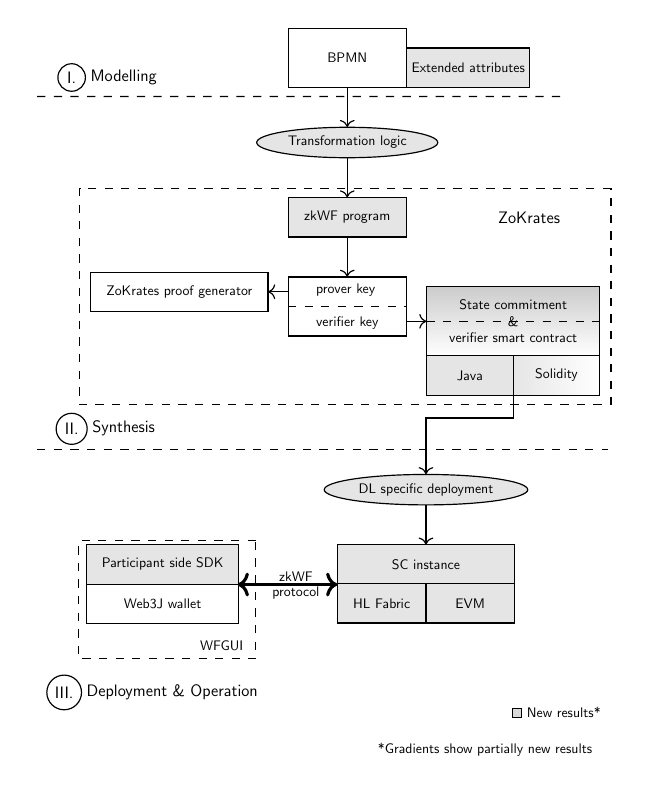
\begin{tikzpicture}[font=\sffamily,line width=0.015cm, scale=0.5,every node/.style={scale=0.5}]
	    \node[rectangle,draw,minimum width= 3cm,minimum height=1.5cm](BPMN){BPMN};
	    \node[rectangle,draw,minimum width= 3cm,minimum height=1cm,right=0 cm of BPMN,xshift=\pgflinewidth,yshift=-0.25cm,fill=gray!20!white,xshift=-\pgflinewidth](ext){Extended attributes};
	    \node[below=0.3 cm of BPMN,xshift=-8cm,yshift=0.5cm] (m1) {};
	    \node[below=0.3 cm of ext,xshift=2.5cm,yshift=0.5cm] (m2) {};
	    \draw[dashed] (m1) -- (m2);
	    \node[above=0.5cm of m1,xshift=1cm,yshift=-1cm,draw,circle](t1){\large{I.}};
	    \node[right=0.5cm of t1,xshift=-1cm]{\large{Modelling}};
	    
	    \node[below=0.5cm of BPMN,draw,ellipse,yshift=0cm,fill=gray!20!white] (transform) {Transformation logic};
	    \draw[<-] (transform.north) -- (BPMN.south);
	    \node[below=0.5cm of transform,draw,rectangle,yshift=-0.0cm,minimum width= 3cm,minimum height=1cm,fill=gray!20!white] (zkwf) {zkWF program};
	    
	    \node[right=1.1cm of zkwf] (zokrates) {\large ZoKrates};
	    
	    \draw[<-] (zkwf.north) -- (transform.south);
	    \node[below=0.5 cm of zkwf,draw,rectangle,yshift=-0.0cm,minimum width= 3cm,minimum height=1.5cm,align=left] (keys) {prover key\\\\ verifier key};
	    \draw[<-] (keys.north) -- (zkwf.south);
	    \draw[dashed] (keys.west) -- (keys.east);
	    \node[left=0.25 cm of keys,draw,rectangle,minimum width=4.5cm,minimum height=1cm,yshift=0.375cm] (proofGen){ZoKrates proof generator};
	    \node[left=0.5cm of keys.west,xshift=1.25cm,yshift=0.375cm] (proverKeyBorder){};
	    \draw[<-] (proofGen.east) -- (proverKeyBorder);
	    \node[right=0.5 cm of keys.east,xshift=-1.25cm,yshift=-0.375cm] (verifierKeyBorder){};
	    \node[right=0.25 cm of keys,align=center,draw,rectangle,minimum width= 4.4cm,minimum height=1.75cm,yshift=-0.375cm,top color=gray!40!white, bottom color=white] (sc) {State commitment\\\&\\verifier smart contract};
	    \draw[<-] (sc.west) -- (verifierKeyBorder);
	    \draw[dashed] (sc.west) -- (sc.east);
	    \node[below=0.5cm of sc,draw,rectangle,yshift=1.0cm,minimum width=2.2cm,minimum height=1cm,xshift=-1.1cm,fill=gray!20!white,yshift=\pgflinewidth] {Java};
	    \node[below=0.5cm of sc,draw,rectangle,yshift=1.0cm,minimum width=2.2cm,minimum height=1cm,xshift=1.1cm,left color=gray!20!white, right color=white,yshift=\pgflinewidth] (solc){Solidity};
	    
	    \node[draw,rectangle,dashed, fit=(zkwf) (solc) (proofGen),minimum width=13.5cm,minimum height=5.5cm]{};
	    
	    \node[below=1.375cm of keys,xshift=-8cm] (s1) {};
	    \node[below=1.375cm of keys,xshift=6.75cm] (s2) {};
	    \draw[dashed] (s1) -- (s2);
	    \node[above=0.5cm of s1,xshift=1cm,yshift=-1cm,draw,circle](t2){\large{II.}};
	    \node[right=0.5cm of t2,xshift=-1cm]{\large{Synthesis}};
	    

	    
	    \node[below=1.75cm of keys,draw,ellipse,fill=gray!20!white,xshift=2cm] (depl) {DL specific deployment};
	    \node[below=0.1cm of sc.south,yshift=0.25cm,xshift=0.0cm] (scBot){};
	    \draw[->] (scBot) -| ++(0,-1.5) -| (depl.north); 
	    
	    \node[below=0.5cm of depl,rectangle,draw,minimum width=4.5cm,minimum height=1cm,fill=gray!20!white](sci){SC instance};
	    \draw[<-] (sci.north) -- (depl.south);
	    \node[below=0 cm of sci,rectangle,draw,minimum width=2.25cm,minimum height=1cm,yshift=\pgflinewidth,xshift=1.125cm,fill=gray!20!white,yshift=\pgflinewidth]{EVM};
	    \node[below=0 cm of sci,rectangle,draw,minimum width=2.25cm,minimum height=1cm,yshift=\pgflinewidth,xshift=-1.125cm,fill=gray!20!white,yshift=\pgflinewidth]{HL Fabric};
	    
	    \node[left=0.5cm of sci,draw,rectangle,xshift=-1.5cm,minimum width=3.85cm,minimum height=1cm,fill=gray!20!white](sdk){Participant side SDK};
	    \node[below=0cm of sdk,rectangle,draw,minimum width=3.85cm,minimum height=1cm,yshift=\pgflinewidth](web3){Web3J wallet};
	    \node[left=0.5cm of sci.south,xshift=-1cm] (sc_side){};
	    \node[right=0.5of sdk.south,xshift=0.655cm] (sdk_side){};
	    \draw[<->,line width=0.04cm] (sc_side) -- (sdk_side);
	    \node[left=0.5cm of sc_side,xshift=0.5cm,yshift=0.2cm,align=center](zkwfp){zkWF};
	    \node[below=0.0cm of zkwfp,yshift=0.1cm]{protocol};
	    \node[below=0.5 cmof web3,yshift=0.7cm,xshift=1.5cm](GUI) {WFGUI};
	    
	    \node[draw,dashed,fit=(sdk) (GUI) (web3),minimum width=4.5cm, minimum height=3cm]{};
	    
	    \node[below=0.5cm of sci,yshift=-2cm,xshift=3.5cm](note){New results*};
	    \node[draw,rectangle,fill=gray!30!white,left=0.5cm of note,xshift=1cm]{};
	    \node[below=0.2cm of note,xshift=-2cm]{*Gradients show partially new results};
	    
	    \node[below=0.5 cm of GUI,xshift=-4cm,yshift=0.5cm,draw,circle](t3){\large{III.}};
	    \node[right=0.5 cm of t3,xshift=-1cm]{\large{Deployment \& Operation}};
	\end{tikzpicture}
	\caption{Toolchain overview}
	 \label{fig:vezerabra}
\end{figure}

%is key-authorized process state changes to be possible only in terms of the smart contract state commitment and stored encrypted state. 
%Note that this goal carries over from the existing state of the art.

%Our \textit{availability goal} is no process external party to stop

%In this paper, we assume the following properties may apply for a given attacker:


%\begin{itemize}
%\item An attacker knows the corresponding BPMN model for a given smart contract instance
%\item A malicious participant may also be an attacker
%\end{itemize}

%Our approach aims at ensuring the following security guarantees.
%\todo{Ezeket befelyezni}
%\begin{itemize}  
% \item Parties not participating cannot modify the state stored on the blockchain
% \item Parties not participating cannot read or guess the current state of the business process execution based on the data stored in the smart contract. 
%\item No party can make an illegal move during the orchestration.
%\item Messages between the participants can be verified.
%\item Participants can identify which party made a given move 
%\end{itemize}

\section{BPMN subset and execution semantics}
%\todo{Intro, subset, extensions}
In this paper, our main focus is on BPMN \textit{collaboration} models. According to the specification, they can contain \textit{processes} or \textit{choreographies}; we work with \textit{collaborative processes}.

Currently, we support a limited but representative set of elements from the BPMN specification, as summarized by table \ref{tab:sup_elem}. Notably, in addition to the Basic Modeling Elements of BPMN 2.0 (see \cite{bpmn}, p28), we also support message throw and catch events, which are of particular importance in collaborative settings. The table denotes those elements as ''stateful'' which have non-instantaneous execution semantics (as declared by the BPMN specification), and these will determine the structure of our execution state vector. In the context of this paper, we will refer to these elements as the ''executable'' ones in the BPMN subset we address.

%Some of the element types are considered executable. Others are there to control the execution flow. Executable elements' (like that of activities) state is tracked by this tool. The currently supported elements can be seen in table \ref{tab:sup_elem}.
\begin{table}
    \centering
    \caption{Supported BPMN modelling elements}
    \begin{tabular}{|c|c|c|}
        \hline
        \textbf{Element name} & \textbf{Notation} & \textbf{Stateful?}\\
        \hline
        \centerTable{Start event}
        &  
\begin{tikzpicture} \node[event] (start) {}; \node[above=0.001 cm of start]{};\node[below=0.001 cm of start]{}; \end{tikzpicture} & \centerTable{no} \\
        \hline
        \centerTable{End Event}  &  
\begin{tikzpicture} \node[end event] (end) {}; \node[above=0.01 cm of end]{};\node[below=0.01 cm of end]{};\end{tikzpicture} & \centerTable{no}\\
        \hline
        \centerTable{Activity} & 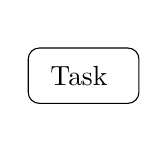
\begin{tikzpicture} \node[task] (task) { Task }; \node[above=0.01 cm of task]{};\node[below=0.01 cm of task]{}; \end{tikzpicture} & \centerTable{yes} \\
        
        \hline
        Sequence flow & \begin{tikzpicture} \draw[-{Stealth[inset=0pt]}] (0,0) -- (1,0);\end{tikzpicture} & no \\
        \hline
        Message flow & \begin{tikzpicture} \draw[-{Stealth[open,inset=0pt]},dashed] (0.05,0) -- (1,0); \node[draw,circle,minimum size=0.1cm,inner sep=0pt, outer sep=0pt] at (0,0) {};\end{tikzpicture} & no \\
        \hline
        \centerTable{Parallel gateway} & 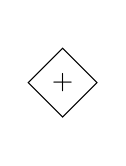
\begin{tikzpicture} \node[gateway,node distance=6emg] (pg) {+}; \node[above=0.01 cm of pg]{};\node[below=0.01 cm of pg]{};\end{tikzpicture} & \centerTable{no} \\
        
        \hline
        \centerTable{Exclusive gateway} & \begin{tikzpicture}
            \node[gateway,node distance=4em,below=of start] (eg) {$\times$};
            \node[above=0.01 cm of eg]{};
            \node[below=0.01 cm of eg]{};
        \end{tikzpicture} & \centerTable{no} \\
        \hline
        Message & \begin{tikzpicture}
            \node[] at (0,0) {\faEnvelope[regular]} ; 
        \end{tikzpicture}& no \\
        \hline
        \centerTable{\makecell{Message Intermediate \\ Catch event  (executable)}} & 
        \begin{tikzpicture}
            \node[intermediate event,below=of eg,xshift=5em] (imc) {\faEnvelope[regular]};
             %\node[above=0.01 cm of imc]{};
             \node[below=0.1 cm of imc]{};
        \end{tikzpicture} & \begin{tikzpicture}
	        \node[](y){yes};
         \node[below=0.2 cm of y]{};
	    \end{tikzpicture}\\
        \hline
	    \centerTable{\makecell{Message Intermediate \\ Throw event  (executable)}} & 
	    \begin{tikzpicture}
		        \node[intermediate event,node distance=2em,below=of imc] (imt) {\faEnvelope};
		        %\node[above=0.01 cm of imt]{};
		        \node[below=0.1 cm of imt]{};
	    \end{tikzpicture} & \begin{tikzpicture}
	        \node[](y){yes};
         \node[below=0.2 cm of y]{};
	    \end{tikzpicture} \\
	    \hline
	    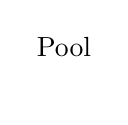
\begin{tikzpicture}
	        \node[](y){Pool};
         \node[below=0.15 cm of y]{};
	    \end{tikzpicture} & 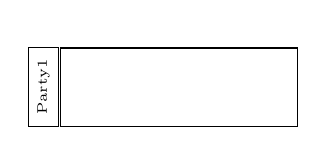
\begin{tikzpicture}[]
	        \node[minimum width=3cm,minimum height=1cm,draw,rectangle](b){};
	        \node[above=0.01 cm of b]{};
	        \node[rotate=90,draw,rectangle,left=0.2cm of b,xshift=0.5cm+\pgflinewidth,yshift=\pgflinewidth,minimum width=1cm] {\tiny Party1};
	    \end{tikzpicture} & \begin{tikzpicture}
	        \node[](y){no};
         \node[below=0.2 cm of y]{};
	    \end{tikzpicture} \\
	    \hline
	    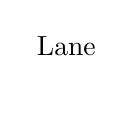
\begin{tikzpicture}
	        \node[](y){Lane};
         \node[below=0.175 cm of y]{};
	    \end{tikzpicture} & 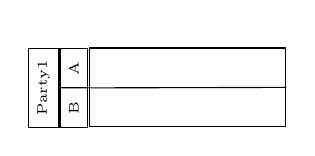
\begin{tikzpicture}[]
	        \node[minimum width=2.5cm,minimum height=1cm,draw,rectangle](b){};
	        \node[above=0.01 cm of b]{};
	        
	        \node[rotate=90,draw,rectangle,left=0.2cm of b,xshift=0.5cm,yshift=-\pgflinewidth,minimum width=0.5cm] (a){\tiny A};
	        \node[rotate=90,draw,rectangle,left=0.2cm of b,xshift=0,yshift=-\pgflinewidth,minimum width=0.5cm] {\tiny B};
	        \node[rotate=90,draw,rectangle,left=0.4cm of a,xshift=0.5cm+\pgflinewidth,yshift=-\pgflinewidth,minimum width=1cm] (p){\tiny Party1};
	        
	        \draw[-] (p.south) --(b.east) ;
	    \end{tikzpicture} & \begin{tikzpicture}
	        \node[](y){no};
         \node[below=0.2 cm of y]{};
	    \end{tikzpicture} \\
	    \hline
    \end{tabular}
    \label{tab:sup_elem}
\end{table}


%We wanted to support at least the Basic Modeling Elements of BPMN 2.0\footnote{See Business Process Model and Notation, v2.0 \cite{bpmn}, page 28.}  to prioritize common components. We have also taken into account making modeling collaborations more executable. This is why We also included Message flows and Intermediate Message events. We chose these elements because these are the ones that are necessary and sufficient to model most of the relevant use cases.

\subsection{BPMN extensions and structural constraints}
%\label{bpmn_attr}
In order to capture properties that are necessary for our zero-knowledge approach, we added two types of extended attributes on top of the existing BPMN specification. On the one hand, a \texttt{zkp:publicKey} attribute is used to separate the tasks of different participants by attaching an EdDSA public key to a pool, a lane, or an executable element. Applying this attribute to an element directly or indirectly (e.g. through inclusion in a pool) is mandatory; however, there are no facilities for key overriding in the model hierarchy yet. The intended usage is to equip either pools or lanes with public keys.

\texttt{zkp:variables} extended attributes can be applied to \textit{activities}. These declare process instance global variables and that the variable may be written by that activity (reads are allowed for all activities). These variables can be used in expressions for exclusive gateways. The gateways support boolean expressions over these global variables.

Some constraints apply to the structure of the BPMN models currently admissible in our scheme.

\begin{itemize}
    \item We support binary gateways (at most two incoming/outgoing edges).
    \item Activities are \textit{atomic}; i.e., subprocesses are not supported.
    \item The model cannot contain loops; sequence and message flows must form a directed acyclic graph.
\end{itemize}

We plan to eliminate these constraints in the future; the required modifications of the state representation and the zkWF program construction are largely incremental.

\subsection{State representation}
Our notion of process instance execution state encompasses the following aspects (for the specific encoding in zkWF programs, please refer to the implementation).

\begin{itemize}
\item A vector $v$ of the current state of executable elements
\item The current values of \textit{global variables}
\item Hashes of the messages already sent in the process
\end{itemize}

Let us represent a business process $M$ as a tuple $(\vertices,\edges,\executables)$, where $\vertices$ is the set of non-flow model elements, $\edges$ is the set of model edges (flows), and $\executables\subset\vertices$ is the set of all executable elements in the business process. Then, $v$ is a vector of $|T|$ size and $\forall v_i \in v$ can have one of the following three values:

\begin{itemize}
    \item 0 (Inactive) -- The element has not been reached yet
    \item 1 (Active) -- The element is ready to be executed or is being executed by a party
    \item 2 (Completed) -- The execution of the element has been completed
\end{itemize}

Note that this state space model is a simplification, especially in terms of the full BPMN activity lifecycle; however, it is a reasonable simplification in the sense that it is of sufficient expressive power for important applications in our context (as we show later). Further research will investigate incorporating the full lifecycle model.

\subsection{Capturing token passing semantics}
As described by the standard, BPMN 2.0 models have token flow-based execution semantics. For the purposes of supporting a different ZKP use case, Aivo et al. \cite{toots_msc} introduce a technique for representing valid BPMN execution state changes through enumerating the possible composite token marking deltas of the elements upon stepping the process. 

Specifically, \cite{toots_msc} introduces an array $P$, where each element of $P$ is a list of token change and element identifier pairs -- essentially, $P$ enumerates the token changes for each allowed stepping of the BPMN model (not unlike Petri net incidence matrices do). 

We construct a very similar $P$ array and embed it into the zkWF program to enable checking whether a proposed state update is valid from the BPMN execution logic point of view.

Our token passing-based operational semantics is the following. Initially, we create a token for every start event and pass it to the first executable element connected to it. Each executable element has one incoming and one outgoing edge. When an executable event has a token, it is marked as ''active''. After completing the execution of the element, the element is marked as ''completed'', and we pass its token to the next executable element -- based on the token holder element's outgoing edge. This approach can be modelled as adding a token ($+1$) when we mark an executable event as ''active'', and we subtract this token ($-1$) when we mark the event as ''done''.

Gateways change the token flow differently. Parallel gateways can split a token on one end and merge them back together on the other end. Exclusive gateways can have many outgoing edges, but only one can be taken based on its assigned expression. A default outgoing edge can also be set, as described in the BPMN specification. End events can have multiple incoming edges but no outgoing edges. They mark the end of a token flow.

To limit the size of our version of array $P$ (necessary to ensure reasonable proof computation times), in our approach, a single step of a model can induce only three token changes at most. (Hence the structural restriction on parallel gateways.) Thus, the array $P$ describing one-step token marking changes for a model $M$ consists of 3-tuples with elements from the set $\mathcal{N}$: 

\begin{align}
    \mathcal{N}&=(+1, -1\}\times T)\cup \{(0,-1)\}
\end{align}

For $T$, we apply a simple integer encoding; the $-1$ in the ''no-token-change'' pair is a don't care placeholder.

%In general, $n\in\mathcal{N}$ is a pair of numbers describing a possible token change. The first component of the pair shows if the token is increased or decreased ($+1$ or $-1$). The second component $i$ marks the token change for the executable event $T[i]$.

%Since not every step consists of three token changes, $n$ can also be an "empty" token change. This is used as a placeholder and is marked as $(0,-1)$.

%Then, $P[i]$ shows how the process state can change in step $i$.

%\subsection{Limitations of BPMN models}
%\label{bpmn_limit}
%As We described in the previous section, "special" BPMN models are needed for the program to work.
%\begin{itemize}
    %\item The model must be a collaboration: It must have at least one pool.
    %\item It only supports a limited subset of the BPMN specification.
    %See section \ref{bpmn_elements}.
    %\item All tasks should have a public key assigned to them. This should be done at the pool/lane level, not individually.
    %\item A parallel gateway can only have two outgoing (and one incoming) edges OR two incoming (and one outgoing) edges. 
    %The reason behind it is described in section \ref{paralhell}. 
    %\item A gateway must be followed by an executable event.
%\end{itemize}

\section{Universal Continuous Mapping} % 2 pages
\label{sec:UCM}
The previous \cref{sec:UE} proposes universal encoding model for various data.
%
Taking that function as a basis, in this section, our Universal Continuous Mapping produces a map of latents to implicitly represent the scene.
We name such scene representation \textbf{Latent Implicit Maps (LIM)}.
%is uesed to produce Latent Implicit Maps 
Which supports surface, surface properties, and high-dimensional surface features. 
%
%\begin{figure}[htbp]
%	\centering
%	\includegraphics[width=.8\linewidth]{im/inherit_graph}
%	\caption{Inheritance graph for the class of Latent Implicit Maps (LIM).}
%	\label{fig:inherit}
%\end{figure}
\begin{figure}[htbp]
	\centering
	\psfragfig[width=1\linewidth]{im/eps/graph}{
		\psfrag{A}{\color{white}{\textbf{BaseMap}}}
		\psfrag{B}{\color{white}{\textbf{SurfaceMap}}}
		\psfrag{C}{\color{white}{\textbf{PropertyMap}}}
		\psfrag{D}{\color{white}{\textbf{LatentMap}}}
	}
	\caption{Inheritance graph for the class of Latent Implicit Maps (LIM).}
\label{fig:inherit}
\end{figure}

%Instead of directly producing a explicit map, our universal continuous mapping produces a map of latents to implicitly represent the scene.
%We name it \textbf{Latent Implicit Maps (LIM)}.
%FIXED: With was used before and should therefore be defined before.



The inheritance graph is plotted in \cref{fig:inherit}.
We design a BaseMap for operating the voxel structure (\cref{sec:map_rep}), dynamically allocating space and fusing maps (\cref{sec:fuse}).
The derived SurfaceMap (\cref{sec:surface_mapping}) and PropertyMap (\cref{sec:context_fields}) process specific data and operate for the specific application.
The LatentMap (\cref{sec:latent_fields}) is derived from PropertyMap.
The main difference is that the PropertyMap mainly operates low dimensional properties, such as color ($c=3$) or infrared ($c=1$) data, etc. 
While the LatentMap operates much higher dimensional feature, such as CLIP embeddings~\cite{ghiasi2022scaling} ($c=768$), for different application purposes.

\subsection{Map Representation}
\label{sec:map_rep}

We follow Neural Implicit Maps (~\cite{huang2021di,yuan2022algorithm,li2022bnv}) to use uniform-spaced voxels to sparsely represent the scene. The scene is $\V V=\{\V v_m = (\V c_m, \V F_m, w_m)\}$. $m$ is the voxel index. $\V v_m$ denotes the contents of that voxel which are $\V c_m\in \mathbb R^3$, $\V F_m\in \mathbb R^{l \times c}$ and $w_m\in\mathbb N$ respectively representing the voxel center, voxel latent feature and observed points count.

With a sequence of incremental frames as input, our model constructs local LIMs (\cref{sec:surface_mapping}, \cref{sec:context_fields}, \cref{sec:latent_fields}) and fuses (\cref{sec:fuse}) into a global LIM.
%
Then the resulting explicit map is inferenced from the global LIM.

\subsection{Surface Mapping}
\label{sec:surface_mapping}

Because the input point cloud $\V X$ is on zero-level of the surface, it is not adequate to recover a 3D field of scene, $f_{SDF}:\mathbb R^3 \rightarrow \mathbb R$.
%
Thus, we explopit the idea of Gaussian Process Implicit Surfaces (GPIS)~\cite{martens2016geometric,lee2019online,wu2021faithful,ivan2022online} to feed derivatives to kernel or to additionally sample non zero-level points.
%And the $\V y$ we use for regression is distance.
%
Both, derivative-based and sample-based GPISs use normal information.
Thus, we first pre-process $\V X$ to obtain normals $\V S$. 

\subsubsection{Using Derivatives based GPIS}
\label{sec:GPIS:deri}

From~\cite{martens2016geometric}, derivatives of a GP are also Gaussian. 
So the covariance between data and derivatives is the differentiation of the covariance function~\cite{solak2002derivative}:
%FIXED: Citation ???
\begin{equation}
	\begin{split}
cov(\frac{f_{SDF}(\V x) }{\partial x_i}, f_{SDF}((x^{'}))) &= \frac{\partial k(\V x, \V x^{'})}{\partial x_i}\\
&=\frac{\partial}{\partial x_i}[f_{posi}(\V x)]^Tf_{posi}(\V x^{'}).
	\end{split}
\end{equation}
Additionally,
\begin{equation}
\begin{split}
cov(\frac{f_{SDF}(\V x) }{\partial x_i}, \frac{f_{SDF}(\V x^{'}) }{\partial x_j}) &= \frac{\partial^2 k(\V x, \V x^{'})}{\partial x_i\partial x^{'}_j}\\
&=\frac{\partial}{\partial x_i}[f_{posi}(\V x)]^T\frac{\partial}{\partial x^{'}_j}[f_{posi}(\V x^{'})].
\end{split}
\end{equation}
So given points $\{\V x_n\}^N_{n=1}$ with normals $\{\V s_n\}^N_{n=1}$ and field values $\{\V y_n=0\}^N_{n=1}$,
the positional encoding function for derivatives is $f_{posi, deri}(\V x, i) = \frac{\partial}{\partial x_i}[f_{posi}(\V x)]$.
Its corresponding field value is the normal value $s_i$ on the axis $i$.
Then,
\begin{multline}
f_{posi, gpis}(\V X)=\\ [f_{posi}(\V X), f_{posi, deri}(\V x, 1), f_{posi, deri}(\V x, 2), f_{posi, deri}(\V x, 3)]
\end{multline}
with regression values $\V y_{gpis}=[\V 0, \V s_{\cdot,1}, \V s_{\cdot,2}, \V s_{\cdot,3}]^T$, where $\V 0 = zeros(1,N)$, $\V s_{\cdot,i}=[\V s_{1,i},\cdots,s_{N,i}]$.

Therefore the local geometric encoding function is
\begin{multline}
f_{enc, GPIS}(\V X, \V y, \V S)=\\
f_{posi, gpis}(\V X)(f_{posi, gpis}(\V X)^Tf_{posi, gpis}(\V X) + \sigma_n^2\V I)^{-1}\V y_{gpis}.
\end{multline}
By introducing derivation into kernels, the matrix size is enlarged 15-times, 
while the encoded feature is still of low dimension $l$:
$F_{\V X, \V y, \V S}=f_{enc, GPIS}(\V X, \V y, \V S)\in \mathbb R^l$.

For inferenceing with the points $\V x_*$, predictions are consistant to \cref{eq:decode}, $y_*=f_{posi}(\V x_*)^T F_{\V X, \V y, \V S}$.

% it extend regression data: $\{\V x_n , )\}^N_{n=1}$ with $\V d_1=(s_{n,1},0,0)$, $\V d_1=(0, s_{n,2}, 0)$, $\V d_3=(0,0,s_{n,3}$ and field values $\{0, \}$

\subsubsection{Using Sample based GPIS}
\label{sec:GPIS:sample}
%Sample based GPIS is more simple.

Sample-based GPIS are mostly used in GPIS researches.
This is because such method does not compute Jacobians and the kernel size can be small.% (e.g. 2 on positive and negative directions each). 
This highly-reduces the processing cost both on time and memory.
%
Given points $\{\V x_n\}^N_{n=1}$ with normals $\{\V s_n\}^N_{n=1}$ and field value $\{\V y_n=0\}^N_{n=1}$,
sample-based GPIS extends the dataset by sample points along the normal direction.
Corresponding field values are the signed distance as the sampled points walk along the normal.
Afterwards, with the extended points and distances $\V X_{ext}$, $\V y_{ext}$, \cref{eq:encode} is applied.
The inference of such model is the same as derivative-based GPIS \cref{sec:GPIS:deri}.

\bigskip

For each frame, points are distributed to its corresponding voxel.
Then we encode the local geometry in voxel using \cref{sec:GPIS:deri} or \cref{sec:GPIS:sample} to obtain $\V v=(\V c, \V F, w)$ with $F\in\mathbb R ^ l$ the geometric latent vector.
Then local LIMs are fused to a global LIM following \cref{sec:fuse}.

To achieve a surface result for visualization, we %follow DI-Fusion to
construct the Signed Distance Field from global LIM by inferring on sample points.
The sample points are from a grid in each voxel with a certain resolution.
By applying the MarchingCube algorithm on SDF, a surface mesh is obtained.


\subsection{Surface Property Fields}
\label{sec:context_fields}

The previous surface mapping (\cref{sec:surface_mapping}) can be considered as a special case of this Surface Property Mapping.
But the two mappings actually do not handling in the same space. 
More precisely for implementation, we do not derive the SurfaceMap class from PropertyMap. 
Instead, as shown in \cref{fig:inherit}, we further introduce a BaseMap to perform the common operations and let them operate specificly on local map construction and visualization, e.g., meshing and coloring.

%Because its surface properties for given point cloud are zero 

%Additionally, it provides a Signed Distance Field as an intermediate for mesh construction. 

We introduce the more general mapping of surface properties.
Since the points are all on zero-level in signed distance fields, the PropertyMap naturally handles in a subspace of $\mathbb R^3$, the surface $\mathcal{S}$.
A surface property in this paper could be any properties for each point, such as color, infrared, and etc.
%
They only differ on $\V y$ in~\cref{fig:encoder} with dimension $c$.

We set the most widely used data color as an example.
Given an observed colored point cloud $\{(\V x_n, \V c_n)|n=0\cdots N\}$ as input, where $\V c_n$ denote the RGB.
Its surface field properties values are $\{\V y_n=c_n\}^N_{n=1}$.
We aggregate the values in two $N\times 3$ matrices $\V X$ and $\V C$.
%
So encoded feature for this point cloud is 
\begin{equation}
\V F_{color}=f_{posi}(\V X)(f_{posi}(\V X)^Tf_{posi}(\V X) +\delta^2_n\V I)^{-1}\V C,
\end{equation}
where $\V F_{color}\in \mathbb R^{l\times 3}$.

Since we use $l=20$ in the approximation function for experiments, the color feature are small.
The color map only stores $20\times3$ float in each voxel for a continuous color field.
%
Note that, our model does not need any training.
It can be directly applied to different types of data.
%
For the inference, because the field is on the surface space, we sample points $\V x_*$ in arbitrary resolution, from the given know mesh or surface construction of a previous surface mapping (\cref{sec:surface_mapping}).
Following~\cref{eq:decode}, the inference points $\V x_*$ are positional-encoded and directly multiplied with color feature $\V F_{color,m}$ in the corresponding voxel $m$ to obtain its value $\V c_{*}=f_{dec}(\V x_{*}, \V F_{color,m})$.

\subsection{Surface Feature Fields}
\label{sec:latent_fields}

Surface Feature Fields are considered as an extensive use of previous Surface Property Fields (\cref{sec:context_fields}).
%
Here we extend the surface properties scope to include features. 
This extension further demonstrates the capability of our mapping model as it is directly used without any training.

Given an embedding function $\phi:\mathbb R^{N\times 3}\rightarrow \mathbb R^{N\times c}$ to process the data $\V X$, we approach the feature of each point as surface properties
$\{\V y_n=\phi (\V X)_{\V x_n}\in \mathbb R^{l\times c}\}^N_{n=1}$.

Following the encoding and fusion as \cref{sec:context_fields} and \cref{sec:fuse}, we construct latent implicit maps for the surface feature fields.
Thus, arbitrary resolutional maps of feature are extracted with $f_{dec}(\cdot, \V F_\cdot)$.

We provide one application in~\cref{sec:openvoc}: Open Vocabulary Scene Understanding. Our model constructs a CLIP space feature field on the surface.
And is therefore able to answer a text input.
The differences compared to Surface Property Fields are demonstrated in~\cref{fig:latent_diff}.
In (c), a CLIP text encoder $f_{text}$ is appended to encode the text command $\pmb u$ to the CLIP feature $\pmb U$.
Considering the left branch produces a surface field for CLIP embeddings, our model is capable to find the wanted region by computing the similarity between features.
\begin{figure}[htbp]
	\centering
	\psfragfig[width=1\linewidth]{im/eps/latent}{
		\psfrag{t}{$f_{text}$}
		\psfrag{xm}{$\V X_m$}
		\psfrag{ym}{$\V y_m$}
		\psfrag{fe}{$f_{enc}$}
		\psfrag{fm}{$f_{im}$}
		\psfrag{Fm}{$\V F_m$}
		\psfrag{x}{$\V x_{*}$}
		\psfrag{y}{$\V y_{*}$}
		\psfrag{fd}{$f_{dec}$}
		\psfrag{u}{$\pmb u$}
		\psfrag{U}{$\pmb U$}
		\psfrag{s}{$score$}
	}
	%\includegraphics[width=1\linewidth]{im/latent}
	\caption{Encoding-decoding diagram in different applications. (a) fold applications directly obtain point properties ($\V y_\text{m}$) from sensor. (b) fold applications achieves point properties with (style, saliency and etc.) function $\phi_{im}$. (c) fold applications use feature as $\V y_\text{m}$ to build a LIM for a (CLIP) feature field. Then a text command is used for extracting the semantic information.}
	\label{fig:latent_diff}
\end{figure}

\subsection{Map Fusion}
\label{sec:fuse}

We follow Neural Implicit Maps~\cite{huang2021di} to update the LIM in a voxel-to-voxel manner:
\begin{equation}
\label{eq:fuse}
\V F_m \leftarrow \frac{\V F_m w_m+\V F^{'}_m w^{'}_m}{w_m+w^{'}_m}, w_m\leftarrow w_m+w^{'}_m,
\end{equation}
where $\V v_m=(\V c_m, \V F_m, w_m)$ and $\V v^{'}_m=(\V c^{'}_m, \V F^{'}_m, w^{'}_m)$ are the voxel $m$ from global and local LIMs respectively.


\begin{figure*}[t]%!ht]
	\abovedisplayskip=0pt
	\abovedisplayshortskip=0pt
	\belowdisplayskip=0pt
	\belowdisplayshortskip=0pt
\centering
\scriptsize
\begin{tabular}{|p{.34\textwidth} p{.20\textwidth} p{.36\textwidth}|} 
\hline
\multicolumn{1}{|c}{\textbf{Verifier} (\vrf)} & & \multicolumn{1}{c|}{\textbf{Prover} (\prv)} \\
\hline
%& & \\

& & 1) When \tcb is invoked (either by \trigger \textbf{[T1]-[T3]} or by a manual call in software), \prv executes \tcb-Att to compute \RA measurement:

\begin{equation*}
	H := \cfattest_\attkey(PMEM, METADATA, \log)
\end{equation*} \\

& & where \attkey is the \RA key pre-shared between \vrf and \vrased~\RA RoT in \prv. Then enter \tcb-Wait.\\

% OAK: we need to send METADATA to \vrf because log pointer is in METADATA and if its not sent, \vrf has to enumerate/guess log pointer, which might not be convenient
3) Receive ($H$, $METADATA$ and \log) and extract $\chal$ from $METADATA$
& \sendmessageleft{top={$\acron$ report}} & 2) In \tcb-Wait: Create and send \acron report $:= H||METADATA||\log$ and wait for approval.\\

& & \\

4) Run verification (including analysis of \log) to determine whether to approve the report:

\begin{equation*}
app:=\vrfy(H, \attkey, PMEM', METADATA, \log)
\end{equation*} & & \\

where $PMEM'$ is the expected software for \prv $PMEM$ and $app \in \{0,1\}$ is an approval bit. & & \\
& & \\
5) Generate a new challenge $\chal'$, a memory region to be monitored ($\er_{min}, \er_{max}$) and an authentication token \auth, where: 

\begin{equation*}
	\auth := \cfattest_\attkey(\chal', \er_{min}, \er_{max}, app)
\end{equation*}

\begin{equation*}
	\chal' := \chal + 1
\end{equation*}
& & \\

6) Create and send \acron response
& & \\
$response := app || \chal' || \er_{min} || \er_{max} || \auth$ & \sendmessageright{top={\acron response}} &  7) In \tcb-Wait: Authenticate the response, producing a one-bit output:

\begin{equation*}
	out := \authen(\attkey, \acron \text{ response})
\end{equation*} \\

& &
Based on $out$ and $app$, it decides the next transition:
\begin{compactitem}
	\item If $out=0$: Re-enter \tcb-Wait. {\it Jump to Step 2}.
	\item Else if $app=0$: Save ($\chal'$, $\er_{min}$ and $\er_{max}$ to $METADATA$) and enter \textit{\tcb-Heal}. {\it Jump to Step 8}.
	\item Else: Save ($\chal'$, $\er_{min}$ and $\er_{max}$) to $METADATA$, exit \tcb and resume execution of $\er$. {\it Jump to Step 9}. 
\end{compactitem}~\\

& & 8) In \tcb-Heal: Execute remediation software (e.g., reboot, reset, software update), then re-start \tcb-Att. {\it Jump to Step 1}. \\

& & \\

& & 9) Resume Application Execution:
    \begin{compactitem}
    \item Whenever executing $\er$: append control-flow transfers to \log.
    \item Whenever a \trigger occurs, \acron causes execution to enter \tcb-Att. {\it Jump to Step 1}.
    \end{compactitem}\\
%& & \\

\hline
\end{tabular}
\vspace{-1em}
\caption{\acron protocol.}
\label{fig:prot}
\vspace{-1.5em}
\end{figure*}


\section{Implementation}
\label{sec:impl}

At \company, we have deployed \sysname in our internal clusters to serve daily DL workloads.
The internal clusters consist of heterogeneous GPUs, including NVIDIA T4 GPU and NVIDIA A10 GPU.
Integrated with Kubernetes~\cite{k8s}, \sysname manages thousands of GPUs in each cluster and more than 20,000 GPUs in all.

\parabf{Service manager.}
For online workloads, we use the existing service manager at \company which deploys containers, discovers service, and autoscales horizontal pods.

\parabf{Global manager.}
We modify the Kubernetes scheduler to schedule offline workloads.
The workload profiler takes several dedicated GPUs, whose number is negligible to the total number of GPUs.
When a new offline workload comes, the workload profiler performs a few dry runs of the workload and utilizes the NVIDIA Data Center GPU Manager (DCGM) tools~\cite{dcgm} and NVIDIA Management Library (NVML)~\cite{nvml} libraries to collect GPU metrics.
We collect about 2,000 data for each GPU type to train the speed predictor.
The MLPs of the speed predictor have four layers with hidden size $64\times 64$.
The MLPs are trained with momentum SGD optimizer~\cite{ruder2016overview} in PyTorch v1.8.0~\cite{paszke2019pytorch} until they converge.
\sysname invokes the scheduler periodically to schedule all offline workloads.
When moving workloads, we record checkpoints of offline workloads and restart the workloads after transmitting the models and checkpoints.
As the datasets are usually colossal, we store the datasets in a remote file system and fetch data during the execution.
We implement the scheduler as a third-party plugin to the Kubernetes scheduler.


\parabf{Local executor.}
Each local executor executes online workloads according to the service manager and offline workloads according to the global manager.
DL workloads are executed in Docker containers with our customized components.
We add Best-Effort GPU DevicePlugin in Kubernetes and relevant control paths with Kubelet and \sysprobe for offline workloads.
To control SM percentage, we leverage the environment variable $CUDA\_MPS\_ACTIVE\_THREAD\_PERCENTAGE$ provided by MPS.
The GPU monitor collects resource metrics through DCGM~\cite{dcgm} and NVML~\cite{nvml} for NVIDIA GPU.
The \sysprobe updates the state machine with the collected resource metrics and empirically-set thresholds.
When the state is unhealthy, the \sysprobe will ask the NodeManager in Kubernetes to evict offline workloads.
\bytecuda intercepts nearly 800 CUDA driver APIs for GPU memory allocation and kernel launch.
The GPU memory quota of offline workloads is fixed to $40\%$ as Figure~\ref{fig:motiv_gpu_resource} reports that most online workloads use less than $60\%$ GPU memory.
We adopt the cpuset of Cgroup for CPU isolation.
For memory, \sysname will evict offline workloads if memory usage is higher than a threshold or the kernel swap daemon is busy for a long time.
The parameters to calculate GPU load in Equation~\ref{equ:gpu_load}$\&$\ref{equ:clock_factor} are empirically selected through trial-and-error.

%\input{content/securityGuarantees.tex}

%


%\section{Choosing a distributed ledger}
The state manager smart contract can run on two different distributed ledgers: 
\begin{enumerate}
    \item Ethereum (or other EVM-compatible ledgers)
    \item Hyperledger Fabric
\end{enumerate}
The verifier part of the smart contract for Ethereum is exported from ZoKrates. For Hyperledger Fabric We used the Zokrates fabric verifier we designed.

%\pagebreak
\begin{tiny}
\begin{table}[h]
    \centering
    %\begin{tabular}{|p{2.25in}p{1.2in}p{1in}p{0.7in}|} 
    \begin{tabular}{|lllcc|} 
    \hline
        Model & Architecture & Dataset & Accuracy & Top ANN Accuracy \\ \hline
        \cite{sparse_spike_gd} & 3 layer SNN & SHD & 77.5 & NA \\ %\hline
        \cite{Kheradpisheh} & 6 layer SNN & MNIST & 98.4 & 99.91 \\ %\hline
        \cite{sparse_spike_gd} & 3 layer SNN & N-MNIST & 97.4 & NA\\ %\hline
        \cite{sparse_spike_gd} & CSNN & F-MNIST & 86.9 & 96.91 \\ %\hline
        \cite{She22} & mMND (SNN) & DVS & 98.0 & NA\\ %\hline
        \cite{Zhang_DigiLiqStateMachine} & Reservoir SNN & TI46 & 99.8 & NA\\ %\hline
        \cite{IMLoss} & ResNet-19 & CIFAR-10 & 95.4 & 99.61 \\ %\hline
        \cite{DSpike} & ResNet-19 & CIFAR-100 & 72.2 & 96.80 \\ \hline
    \end{tabular}
\end{table}
\end{tiny}


\pagebreak
\begin{tiny}
\begin{table}[h]
    \centering
    %\begin{tabular}{|p{2.25in}p{1.2in}p{1in}p{0.7in}|} 
    \begin{tabular}{|lllc|} 
    \hline
        Model & Architecture & Dataset & Accuracy \\ \hline
        \cite{sparse_spike_gd} & 3 layer SNN & SHD & 77.5 \\ %\hline
        \cite{Kheradpisheh} & 6 layer SNN & MNIST & 98.4 \\ %\hline
        \cite{sparse_spike_gd} & 3 layer SNN & N-MNIST & 97.4 \\ %\hline
        \cite{sparse_spike_gd} & CSNN & F-MNIST & 86.9 \\ %\hline
        \cite{She22} & mMND (SNN) & DVS & 98.0 \\ %\hline
        \cite{Zhang_DigiLiqStateMachine} & Reservoir SNN & TI46 & 99.8 \\ %\hline
        \cite{IMLoss} & ResNet-19 & CIFAR-10 & 95.4 \\ %\hline
        \cite{DSpike} & ResNet-19 & CIFAR-100 & 72.2 \\ \hline
    \end{tabular}
\end{table}
\end{tiny}

\pagebreak
\begin{tiny}
\begin{table}[h]
    \centering
    %\begin{tabular}{|p{1.25in}p{1.2in}p{1in}|} 
    \begin{tabular}{|lcc|} 
    \hline
        Dataset & Frequency & Percent \\ \hline
        \textbf{MNIST} & \textbf{41} & \textbf{24.8} \\ %\hline
        N-MNIST & 5 & 3.0 \\ %\hline
        F-MNIST & 6 & 3.6 \\ %\hline
        DVS & 7 & 4.2 \\ %\hline
        ImageNet & 19 & 11.5 \\ %\hline
        \textbf{CIFAR-10} & \textbf{55} & \textbf{33.3} \\ %\hline
        CIFAR-100 & 24 & 14.5 \\ %\hline
        All Others & 6 & 3.6 \\ \hline
    \end{tabular}
\end{table}
\end{tiny}

%\section{Implementation?}

\section{Results}
\label{results}

\begin{figure*}[ht]
    \centering
    \includegraphics[scale=0.15,trim={0 2.5cm 0 5cm},clip]{images/aoi-single_burst}
    \caption{The time average peak Age of Information with burst and \gls{soa} loss values against the dynamic reliability logic for different network topologies.}
    \label{fig:aoi_burst}\vspace{-0.4cm}
\end{figure*}


This paper focuses on both transport layer and application layer metrics to determine the feasibility of dynamic reliability. For this, we have selected the session packet volume, as transmitted, retransmitted, lost and backlogged packets as \glspl{kpi} for the transport layer; while focusing on the \gls{aoi} for the application layer. The \gls{aoi} was chosen as a crucial indicator for the freshness of packets in real-time applications. More specifically, this work adopts the time average peak \gls{aoi} equation \cite{aoi_equation} depicted in Eq. \ref{aoi}, where $\Delta(r_{i+1})$ is the $i$th update at the time it was received at the server, for a session time period of $\tau$.

\begin{equation}
    \label{aoi}
    \gls{aoi}_\tau = \frac{1}{n-1}\sum_{i=1}^{n-1} \Delta(r_{i+1})
\end{equation}

We include a comparison between the vanilla QUIC implementation which does not enjoy the dynamic reliability extension, with a number of dynamic reliability policies. The tests were run a number of times for statistical significance, with the mean value of vanilla implementation used as a baseline for comparison. The topology utilised both random loss and bursty loss to explore the bounds of dynamic reliability. The \gls{soa} loss in the figures correspond to the loss values presented in Table. \ref{tab:path_char}, for ease of comparison between bursty and random loss scenarios.

\subsection{Transport-Layer KPIs}

To analyse the performance gain at the transport layer due to dynamic reliability, the volume of transmitted and backlogged packets is examined. The figures are in the form of boxplots, which take the vanilla implementation as a benchmark, depicted as the red dashed line.

As seen in Fig. \ref{fig:sent_burst}, the loss plays a crucial role in the performance of the reliability policies. The policies under random loss did incredibly well for the networks with a larger capacity, namely \gls{mmwave} and Sub-6~GHz, whereas for burst loss, the lower network capacities had a larger packet reduction. With the increase in burst loss, the behaviour of the set split reliable policies became unpredictable, if a reliable assignment happened to coincide with a burst loss, the number of transmitted packets increases, and vice versa. On the other hand, in smarter policies, such as Loss-Aware, the performance lightly matched the vanilla baseline, as the reliable assignment dominated the session to compensate for a higher burst loss. Not only that but, the burst loss also impacted the variance of the transmitted packets for the policies.

Unsurprisingly, the unreliable focused policy, 80-20 split, outperformed other policies for all topologies in random and bursty loss scenarios, with an approximate reduction of 80\%. That being said, the majority of the policies reduced the transmitted packets on the link by approximately 70\% for random loss, while the reduction started at $\approx 15\%$ and decreased as the loss increased for the burst loss scenario.

The retransmitted and lost packets, not shown due to space limitations, followed the same trend as the transmitted packets for the random loss scenarios. However, for the burst loss scenarios, the larger capacity networks had a lower reduction in the retransmitted and lost packets. This can be seen as a favorable outcome since the lower capacity networks are scarce on resources. It is important to note that the Loss-Aware policy mimicked the vanilla approach as the burst loss increased, signifying the overwhelming appointment of reliable packets in adapting to the harsh burst loss conditions.
 
Alternatively, Fig. \ref{fig:backlog_burst} clearly shows a stark comparison between the policies and loss scenario in the reduction of the backlogged packets. The Loss-Aware policy for random loss scenario reduced the backlogged packets by up to 50\%, beating all other policies by approximately 30\%. Furthermore, it is clear that the unreliability focused policies resulted in the lowest backlog for the session. In comparison, we notice that the burst loss and the backlogged frequency have a positive correlation, where the maximum reduction of the backlogged packets for the policies is at most 20\%. Much like the transmitted packets, the probability of a burst loss occurrence plays a vital role in the number of retransmissions sent and by extension the number of backlogged packets. Thus, we can conclude that the stress placed on the buffer is a result of the reliable packets which is tightly coupled with the congestion on the session. Whereas, unreliable focused policies did not encounter such a phenomenon regardless if it was experiencing a burst loss.


\subsection{Application-Layer KPIs}

The feasibility of dynamic reliability for real-time applications can be determined by the \gls{aoi}, with comparison across different topologies and policies. If we take a strict approach and consider anything below $10$~ms is real-time \cite{real-time}, then all the reliability policies passed that requirement, which is attractive for real-time applications, as shown in Fig. \ref{fig:aoi_burst}. Utilising the median as an estimate of the runs, the policies in the WLAN and Sub-6~GHz topology with random loss floated around $4-5$~ms with negligible difference, while the \gls{aoi} for \gls{mmwave} was $\approx 2-3$~ms. It is clear that the \gls{aoi} and the network capacity have a negative correlation, as the network capacity decreases, the \gls{aoi} increases. The same correlation is extended to the bursty loss scenarios, where \gls{mmwave} dominated the other topologies. That being said, it is crucial to note that the \gls{aoi} for the reliability policies is often slightly better than or equal to the \gls{aoi} of the vanilla implementation, proving that dynamic reliability reduces the congestion of the session at no cost to the \gls{aoi}.



\section{Limitations and Future Work}

We summarize the limitations we have identified for our method and propose
future research directions.

\textbf{Parallel implementation:} 
With a focus on accuracy and algorithms, our implementation for this work is
serial. Some of the most time-consuming routines in our method can easily
benefit from a parallel implementation, while the same is not obvious for the
SAP solver and the Schur complement computation. Leveraging the power of
parallelization on modern hardware for these computations is an interesting area
for future investigation.

\textbf{Rotational invariance:} 
As with all other linear constitutive models, our linearized model with lagged
rotational component is not rotationally invariant. Thus it is not suitable for
simulation of extreme deformations using large time steps. For those scenarios,
we fall back to traditional nonlinear models with Hessian positive definite
corrections proposed in \cite{bib:teran2005robust}.

\textbf{Self-contact:} 
We do not consider self-contact at the moment due to the lack of support by our
geometry engine. Self-contact can be incorporated into our method by updating the
geometry engine to augment the set of contacts reported.

\textbf{Tunneling at high speeds:} Though our method has a lower computational
cost, it could benefit from continuous collision detection strategies
\cite{bib:li2020ipc} to provide constraints before contact is established. This
would allow to mitigate issues such as objects tunneling past each other at high
speeds. Efficient solution to mitigate this issue is a topic of active research
for the authors.

\textbf{Redundant constraints:} Our geometry engine often introduces a large
number of constraints to resolve contact. Similarly, welding a large number of
deformable mesh vertices to a rigid body (as done in Section
\ref{sec:bubble_gripper}) introduces many constraints. Even though our SAP
solver \cite{bib:castro2022unconstrained} provides existence and uniqueness
guarantees, a large number of constraints hurts performance as can be observed
in the \emph{Soft-bubble} example. We are currently investigating strategies to
significantly reduce the number of constraints without sacrificing accuracy.


\section{Conclusion}\label{sec:conclusion}
In this work, we focus on addressing the fundamental challenge of OOD detection tasks, which is how to fully understand the semantic discrepancy between the ID/OOD samples. We reveal that the key to success in the realistic SCOOD task is to allocate as many ID samples in the unlabeled set correctly as possible. To this end, we propose a novel uncertainty-aware optimal transport scheme that introduces class-specific energy scores as guidance for effective label assignment. Experimental results show that our method achieves better performance than previous state-of-the-art methods on SCOOD benchmarks.

\textbf{Limitations.} In addition to temperature scaling, other techniques such as feature clipping applied in ReAct~\cite{sun2021react} also enhance the performance of energy score, so how to obtain an OOD score that best fits the SCOOD task can be further explored. Moreover, a setting highly related to SCOOD has been proposed in \cite{katz2022training} and formulated as a constrained optimization problem. We will also theoretically analyze these practical OOD settings in our feature work.

% \section*{Acknowledgments}
\textbf{Acknowledgments.} 
This work is supported by National Key R\&D Program of China under Grant 2020AAA0105701, National Natural Science Foundation of China (NSFC) under Grants 61872327, Major Special Science and Technology Project of Anhui, National Natural Science Foundation of China (62033012) and Ant Group through Ant Research Intern Program.


\section*{Acknowledgment}
This work was partially created under, and financed through, the Cooperation Agreement between the Hungarian National Bank (MNB) and the Budapest University of Technology and Economics (BME).
%The preferred spelling of the word ``acknowledgment'' in America is without
%an ``e'' after the ``g''. Avoid the stilted expression ``one of us (R. B.
%G.) thanks $\ldots$''. Instead, try ``R. B. G. thanks$\ldots$''. Put sponsor
%acknowledgments in the unnumbered footnote on the first page.

%\section*{References}

%Please number citations consecutively within brackets \cite{b1}. The
%sentence punctuation follows the bracket \cite{b2}. Refer simply to the reference
%number, as in \cite{b3}---do not use ``Ref. \cite{b3}'' or ``reference \cite{b3}'' except at
%the beginning of a sentence: ``Reference \cite{b3} was the first $\ldots$''
%
%Number footnotes separately in superscripts. Place the actual footnote at
%the bottom of the column in which it was cited. Do not put footnotes in the
%abstract or reference list. Use letters for table footnotes.
%
%Unless there are six authors or more give all authors' names; do not use
%``et al.''. Papers that have not been published, even if they have been
%submitted for publication, should be cited as ``unpublished'' \cite{b4}. Papers
%that have been accepted for publication should be cited as ``in press'' \cite{b5}.
%Capitalize only the first word in a paper title, except for proper nouns and
%element symbols.
%
%For papers published in translation journals, please give the English
%citation first, followed by the original foreign-language citation \cite{b6}.

\bibliography{refs/mybib}


\begin{IEEEbiography}[{\includegraphics[width=1in,height=1.25in,clip,keepaspectratio]{img/balazs.JPG}}]{Balázs Ádám Toldi}
received  his BSc in computer engineering in 2023 from the Budapest University of Technology and Economics (BME). Currently, he is an MSc student at BME, with a primary specialization in cybersecurity and a secondary specialization in critical systems.
\end{IEEEbiography}
\begin{IEEEbiography}[{\includegraphics[width=1in,height=1.25in,clip,keepaspectratio]{img/kiskep2.png}}]{Imre Kocsis} received his PhD from the Budapest University of Technology and Economics (BME) in 2019. Currently, he serves as a senior lecturer and leading blockchain researcher at the Critical Systems research group of the Dept. of Measurement and Information Systems of BME. He leads the activities of the group in conjunction with the Hyperledger Foundation and the university's participation in the European Blockchain Services Infrastructure (EBSI) network.
\end{IEEEbiography}
%\begin{thebibliography}{00}
%    \bibitem{b1} G. Eason, B. Noble, and I. N. Sneddon, ``On certain integrals of Lipschitz-Hankel type involving products of Bessel functions,'' Phil. %Trans. Roy. Soc. London, vol. A247, pp. 529--551, April 1955.
%    \bibitem{b2} J. Clerk Maxwell, A Treatise on Electricity and Magnetism, 3rd ed., vol. 2. Oxford: Clarendon, 1892, pp.68--73.
%    \bibitem{b3} I. S. Jacobs and C. P. Bean, ``Fine particles, thin films and exchange anisotropy,'' in Magnetism, vol. III, G. T. Rado and H. Suhl, Eds. %New York: Academic, 1963, pp. 271--350.
%    \bibitem{b4} K. Elissa, ``Title of paper if known,'' unpublished.
%    \bibitem{b5} R. Nicole, ``Title of paper with only first word capitalized,'' J. Name Stand. Abbrev., in press.
%    \bibitem{b6} Y. Yorozu, M. Hirano, K. Oka, and Y. Tagawa, ``Electron spectroscopy studies on magneto-optical media and plastic substrate interface,'' %IEEE Transl. J. Magn. Japan, vol. 2, pp. 740--741, August 1987 [Digests 9th Annual Conf. Magnetics Japan, p. 301, 1982].
%    \bibitem{b7} M. Young, The Technical Writer's Handbook. Mill Valley, CA: University Science, 1989.
%\end{thebibliography}
\vspace{12pt}

%\section{Remaining TODO}
%\begin{itemize}
%    \item "Nemgagyi" video
%    \item Table I cleanup
%    \item Fix Table I: \url{https://tex.stackexchange.com/questions/152067/tikz-picture-in-table}
%    \item Specify nature of randomness
%    \item Modellt lelevelezni
%    \item Publishers for the references
%    \item Checking the title casing for the references
%\end{itemize}

\end{document}
